\section{Extruding PLA with Barium Sulfate\label{sec:methodology:extrudingBaSO4}}

The overall goal of the research team is to incorporate barium sulfate (BaSO\textsubscript{4}) into PLCL via extrusion. Barium sulfate provides contrast in imaging to allow the device to be easily identifiable via imaging modalities.

Because PLCL extrusion is still being refined (see Section~\fullref{sec:methodology:extrudingPLCL}), PLA was used as a base material for initial methodology testing and refinement. PLA is a standard material for extrusions, which allows for more streamlined research of barium sulfate effects by eliminating potential confounding variables.

The goal of this research was to assess the effects of barium sulfate on extrudability, printability, and mechanical properties in an effort to determine the optimal percentage of barium sulfate required in the final device.

\subsection{Sample Preparation\label{sec:methodology:extrudingBaSO4:samplePrep}}

Material was prepared by following methodologies established in existing literature and guidance from 3Devo customer support~\cite{RefWorks:RefID:62-ning2015additive,RefWorks:RefID:396-3devotroubleshooting}.

This involved weighing PLA pellets, coating the pellets in mineral oil to improve barium sulfate adhesion, and mixing in barium sulfate.

\subsubsection{Measuring Percent Composition\label{sec:methodology:extrudingBaSO4:samplePrep:percentComp}}

Percent composition of the final sample was tracked through a Microsoft Excel sheet. Compositions of 0\%, 2.5\%, 5\%, 7.5\%, and 10\% barium sulfate were created. For each sample group, roughly $1g$ of mineral oil was added based on recommendations from 3Devo customer support.

Initially, the weight of barium sulfate required was based on the weight of PLA following Equation~\eqref{eq:simplifiedBaSO4PercentComp}. For example, if $100g$ of PLA were used, a 5\% composition of barium sulfate mixture would require $5g$ of barium sulfate.

\begin{equation}
        BaSO_4 (g) = (Desired Percent) * (PLA (g))
        \label{eq:simplifiedBaSO4PercentComp}
\end{equation}

This method does not take into account the total weight of the mixture. Following the previous example, $5g$ of barium sulfate with $100g$ of PLA would be 4.78\% rather than 5\% based on Equation~\eqref{eq:adjustedBaSO4PercentComp}.

\begin{equation}
        BaSO_4 (\%) = \frac{BaSO_4 (g)}{BaSO_4(g) + PLA(g)}
        \label{eq:adjustedBaSO4PercentComp}
\end{equation}

As a result, samples were remade using this updated measurement technique to account for the weight of all materials as shown in Equation~\eqref{eq:finalBaSO4PercentComp}.

\begin{equation}
        BaSO_4 (\%) = \frac{BaSO_4 (g)}{BaSO_4(g) + PLA(g) + Oil(g)}
        \label{eq:finalBaSO4PercentComp}
\end{equation}

Equation~\eqref{eq:finalBaSO4PercentComp} can be rearranged to solve for the required weight of barium sulfate based on the desired percentage and predetermined weights of PLA and mineral oil. This rearrangement is shown below in Equation~\eqref{eq:requiredWeightOfBaSO4}.

\begin{equation}
        BaSO_4(g) = \frac{BaSO_4(\%) * (PLA(g) + Oil(g))}{1-BaSO_4(\%)}
        \label{eq:requiredWeightOfBaSO4}
\end{equation}

\subsubsection{Preparing Barium Sulfate\label{sec:methodology:extrudingBaSO4:samplePrep:preparingBariumSulfate}}

Initially, the barium sulfate was poured directly from its container. This led to large clumps of barium sulfate within the mixture and in turn large clumps of material in the extruded filament.

Based on these findings and existing literature, the barium sulfate was first crushed using a mortar and pestle before being incorporated into the mixture~\cite{RefWorks:RefID:77-hamedani2018threedimensional}.

\subsubsection{Creating Sample Mixtures\label{sec:methodology:extrudingBaSO4:samplePrep:creatingSampleMixtures}}

To begin preparing samples, a plastic beaker was washed and dried. PLA pellets were then poured into the beaker followed by roughly $1g$ of mineral oil. Weights of each material were entered into a Microsoft Excel sheet to determine the required amount of barium sulfate following Equation~\eqref{eq:requiredWeightOfBaSO4}.

The PLA/oil mixture was stirred by covering and rotating the beaker. Once the PLA pellets were adequately coated in oil, barium sulfate was added to the mixture. This was all combined again by covering and rotating the beaker.

Table~\ref{tab:methodology:extrudingBaSO4:sampleMixtures} summarizes the mixtures created for testing.

\begin{table}[h!]
        \centering
        \caption{Sample mixtures of PLA/Barium sulfate.}
        \label{tab:methodology:extrudingBaSO4:sampleMixtures}
        \begin{adjustbox}{max width=\textwidth}
                \begin{tabular}{c c c c c c p{4cm}}
                        \hline
                        Base Material Weight (g) & Desired BaSO$_4$ (\%) & Actual BaSO$_4$ (\%) & Required Amount of BaSO$_4$ (g) & Mineral Oil (g) & Barium Sulfate (g) & \% Composition                              \\
                        \hline
                        66.068                   & 2.50                  & 2.51                 & 1.694                           & 0.642           & 1.703              & PLA: 96.57\%, BaSO$_4$: 2.49\%, Oil: 0.94\% \\
                        100.02                   & 5.00                  & 4.84                 & 5.264                           & 1.115           & 5.092              & PLA: 94.16\%, BaSO$_4$: 4.79\%, Oil: 1.05\% \\
                        50.009                   & 7.50                  & 7.54                 & 4.055                           & 1.059           & 4.080              & PLA: 90.68\%, BaSO$_4$: 7.40\%, Oil: 1.92\% \\
                        50.013                   & 10.00                 & 10.02                & 5.557                           & 0.748           & 5.568              & PLA: 88.79\%, BaSO$_4$: 9.88\%, Oil: 1.33\% \\
                        \hline
                \end{tabular}
        \end{adjustbox}
\end{table}

An example of a sample mixture is shown below in Figure~\ref{fig:methodology:extrudingBaSO4:exampleMixture}

\begin{figure}[h!]
        \centering
        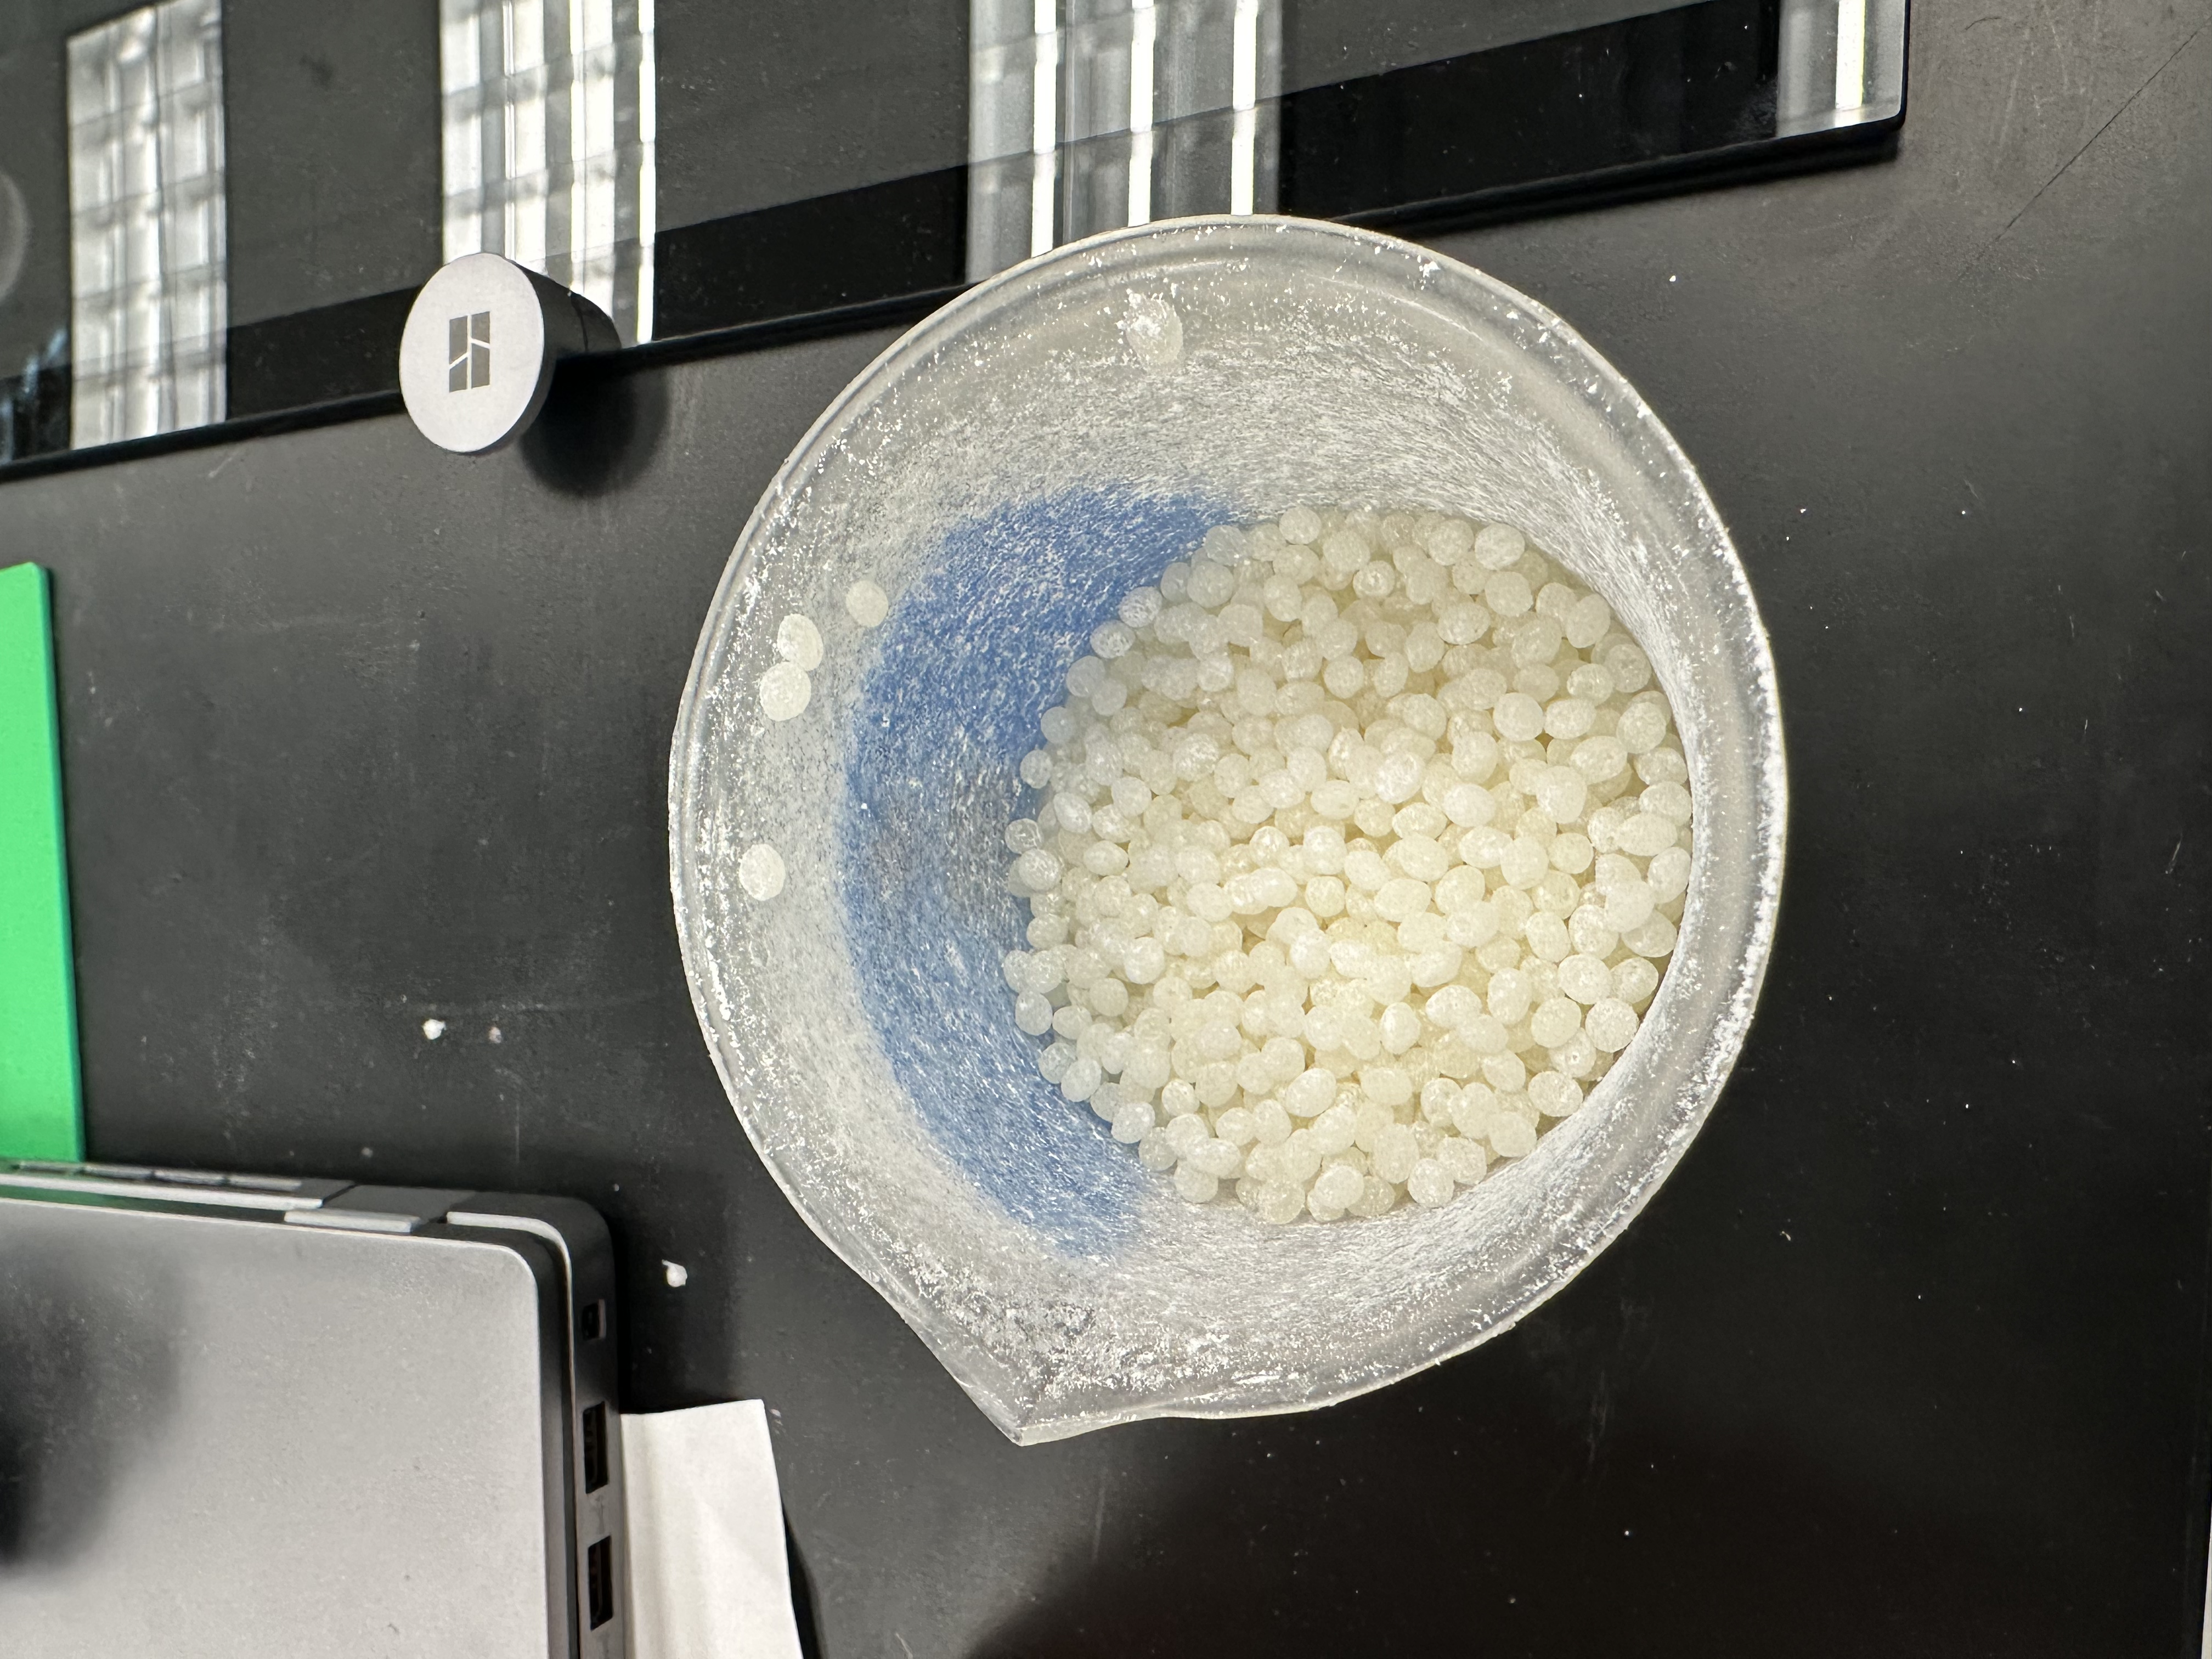
\includegraphics[width=0.5\linewidth]{../figs/methodology/baSO4Extrusions/example_mixture.png}
        \caption{Example of PLA and Barium Sulfate mixture.}
        \label{fig:methodology:extrudingBaSO4:exampleMixture}
\end{figure}

\subsection{Sample Extrusion\label{sec:methodology:extrudingBaSO4:sampleExtrusion}}

Following guidance from 3Devo customer support, the samples were initially extruded at PLA presets - 170, 185, 190, 170 (\textcelsius) - and 4 RPM. If adjustments were necessary, 3Devo customer support suggested raising all heat zones by 5\textcelsius ~at a time to maintain the same relative temperature profile.

Results and discussion of the PLA/BaSO\textsubscript{4} extrusions can be found in ~\fullref{sec:results:extrudingBaSO4} and~\fullref{sec:results:extrudingBaSO4} respectively.
